\documentclass[8pt]{beamer}

\usepackage[utf8]{inputenc}
\usepackage[T1]{fontenc}

\usepackage{longtable}
\usepackage{booktabs}

\usepackage{graphicx}
\usepackage{subfig}
\usepackage{floatrow}
\captionsetup{labelsep=period}

\usepackage[]{algorithm2e}

\usepackage{standalone}

\usepackage{amssymb, amsmath, mathrsfs, mathtools, dsfont, bbold}

\usetheme{ign}

\title{Classification et apprentissage statistique}
\subtitle{Supervisé et non-supervisé}
\author{Oussama ENNAFII}
\institute{ENSG}
\date{\today}

\begin{document}

	\begin{frame}[plain]
		\titlepage{}
	\end{frame}

	\section{Introduction}
		\begin{frame}{Classification: première définition}
			Champs lexical de classer:
			\begin{itemize}
				\item<2-> ranger,
				\item<3-> labeliser,
				\item<4-> catégoriser,
				\item<5-> hiérarchiser.
			\end{itemize}
			\uncover<6->{
				\begin{block}{Esquisse de définition}
					Classer: ranger \(n\) \textbf{objets} dans \(k\) \textbf{catégories} (avec \(k \ll n\)).
				\end{block}
			}
		\end{frame}
		
		\begin{frame}{Comment classer?}
			\begin{itemize}
					\item<1-> Comment caractériser un objet à classer?
					\item<2-> Comment sont-elle définit les catégories (ou classes) d'objets?
			\end{itemize}
		\end{frame}
	
	\section{Classification}
		\subsection{Exemples}
			\begin{frame}{Reconaissance d'objet}
				\begin{figure}[H]
					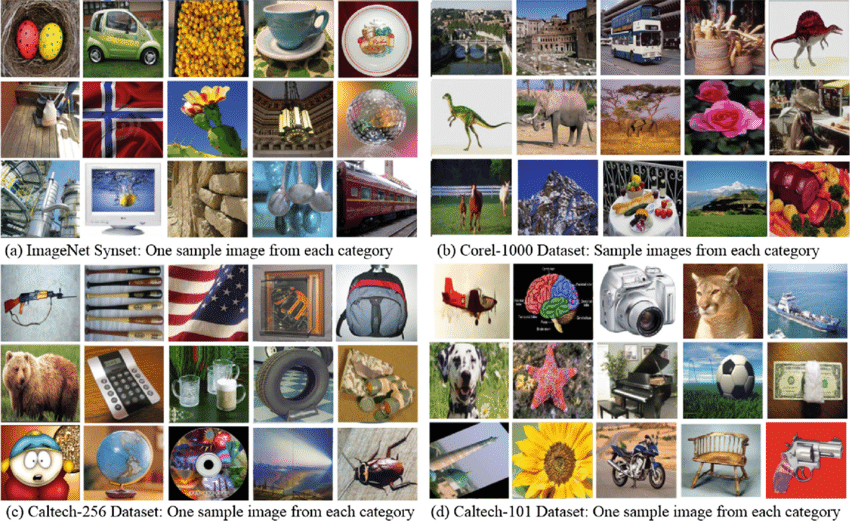
\includegraphics[width=.7\textwidth]{images/samples/image_datasets}
					\caption*{\tiny Exemples de base de données d'images~\cite{ahmed2017fusion}.}
				\end{figure}
			\end{frame}
			
			\begin{frame}{Occupation du sol}
				\begin{figure}[H]
					\ffigbox[\FBwidth]
					{
						\begin{subfloatrow}[2]
							\ffigbox[\FBwidth]
							{
								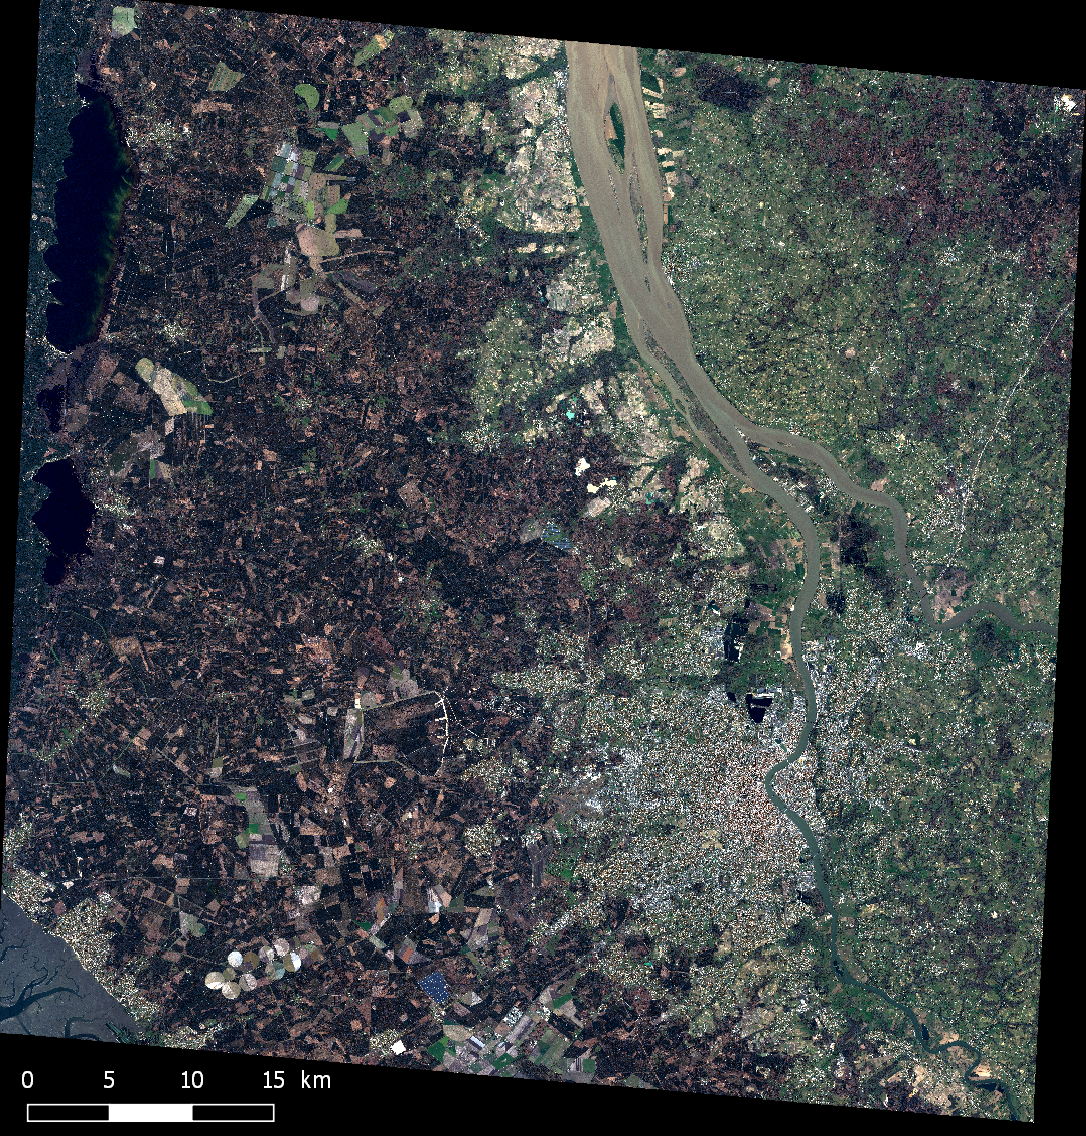
\includegraphics[width=.31\textwidth]{images/samples/gironde}
							}
							{
								\caption*{\tiny Image de la Gironde prise par SPOT en 2016: Résolution 1.5m, 4 canaux: \{{\color{purple!20}Infrarouge}, {\color{red}Rouge}, {\color{green}Vert}, {\color{blue}Bleu}\}.}
							}
							\ffigbox[\FBwidth]
							{
								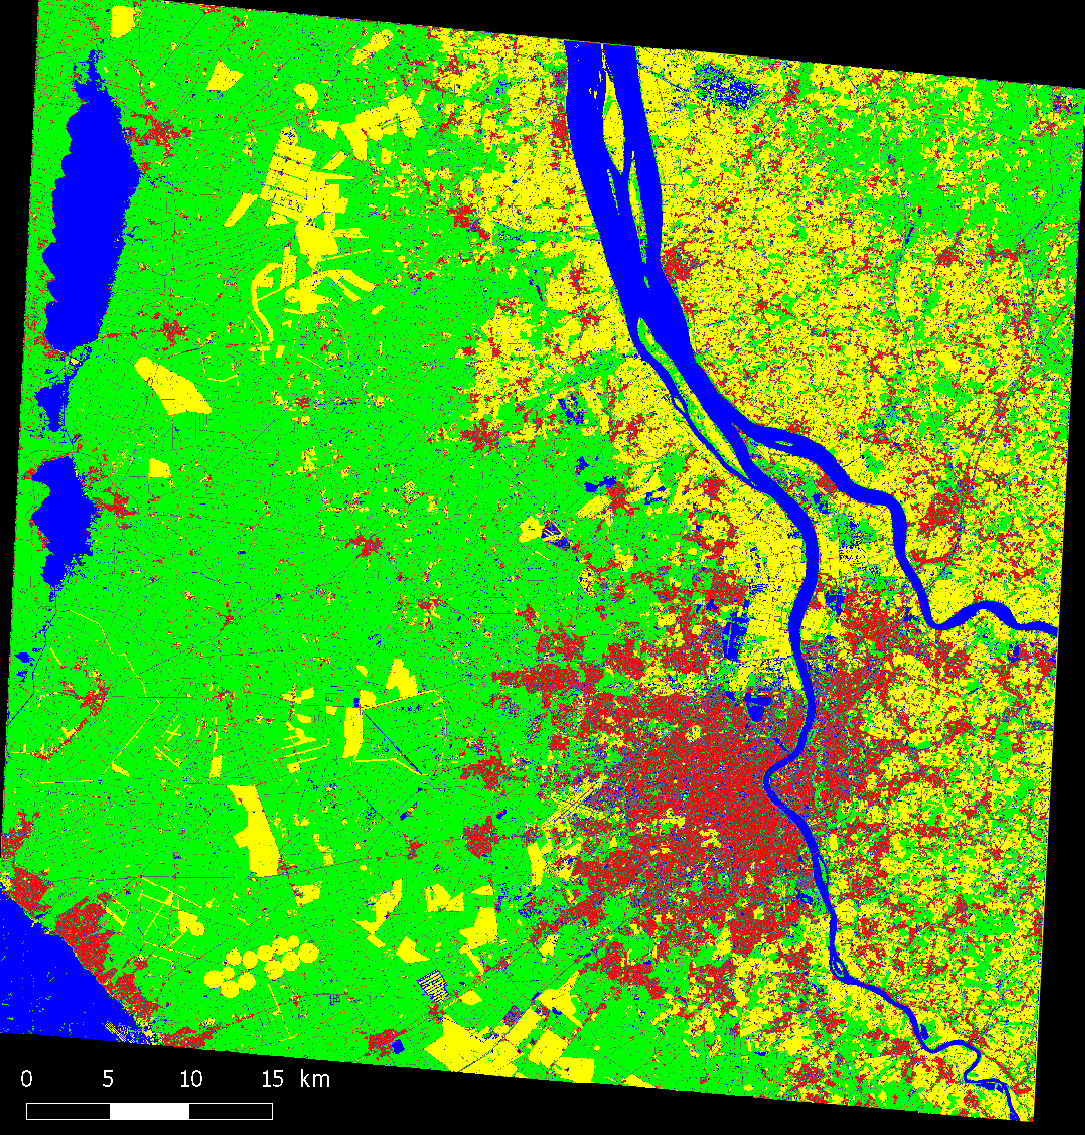
\includegraphics[width=.31\textwidth]{images/samples/gironde_classif}
							}
							{
								\caption*{\tiny Occupation des sols extraite de l'image: {\color{red}\(\blacksquare\)} Bâti, {\color{green}\(\blacksquare\)} Forêt, {\color{yellow}\(\blacksquare\)} Culture, {\color{gray}\(\blacksquare\)} Routes, {\color{blue}\(\blacksquare\)} Eau.}
							}
						\end{subfloatrow}
					}
					{
						\caption*{\tiny Classification appliquée pour l'Occupation des sols~\cite{postadjian2017investigating}.}
					}
				\end{figure}
			\end{frame}

			\begin{frame}{Segmentation de nuage de points}
				\begin{figure}[H]
					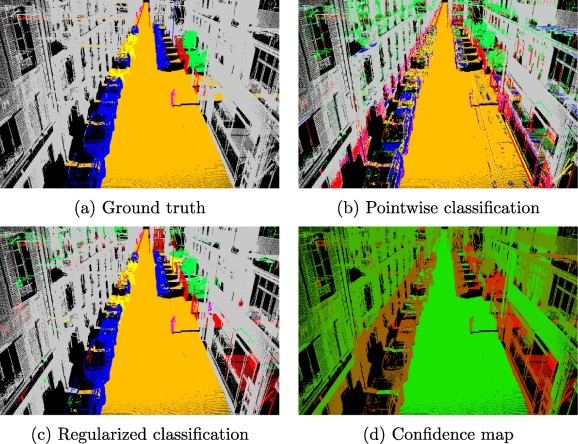
\includegraphics[width=.6\textwidth]{images/samples/pc_classification}
					\caption*{\tiny Exemple de classification de nuage de point\cite{landrieu2017structured}.}
				\end{figure}
			\end{frame}

			\begin{frame}{Détection de phénomènes}
				\begin{figure}[H]
					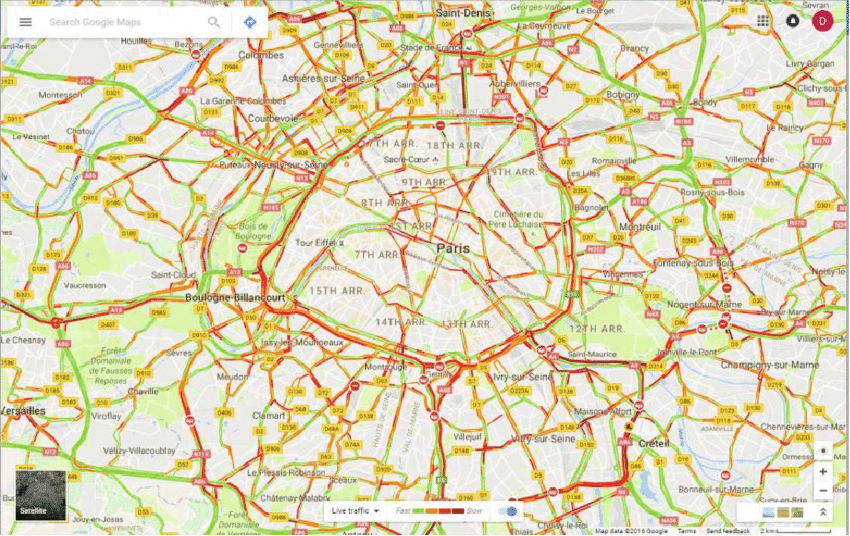
\includegraphics[width=.65\textwidth]{images/samples/traffic_paris}
					\caption*{\tiny Exemple de classification utilisé pour déterminer les conditions de circulation à Paris le 06/09/2016 à 9:30~\cite{tutic2016google}.}
				\end{figure}
			\end{frame}

			\begin{frame}{Classification avec RADAR}
				\begin{figure}[H]
					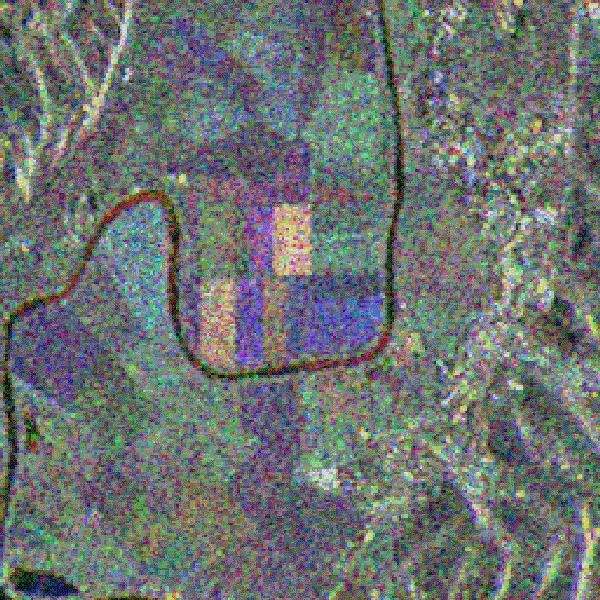
\includegraphics[width=.45\textwidth]{images/samples/radar}
					\caption*{\tiny Exemple d'occupation de sol utilisant basée RADAR~\cite{EsaRadar}.}
				\end{figure}
			\end{frame}

		\subsection{Observations}
			\begin{frame}{Comment caractériser les observations?}
				\begin{itemize}
					\item<1-> Comment sont représentés les données à classer?
					\item<2-> Quel est le point commun entre ces observations?
				\end{itemize}
			\end{frame}
		
			\begin{frame}{Observations}
				Les observations peuvent prendre beaucoup de formes:
				\begin{itemize}
					\item<2-> Image;
					\item<3-> Série temporelle (son, vidéo \dots);
					\item<4-> Graph de données;
					\item<5-> Nuage de points (LIDAR par exemple).
				\end{itemize}
			\end{frame}

			\begin{frame}{Attributs: représentation vectorielle}
				\begin{itemize}
					\item<1-> On représente généralement les observables par un vecteur dans \(\mathbb{R}^d\) qu'on nome attributs.
					\item<2-> On notera la \(i\)-ème observation par \(X^i = \begin{pmatrix}
						X^i_1\\
						X^i_2\\
						\vdots\\
						X^i_d
					\end{pmatrix}\).
					\item<3-> On notera donc l'ensemble des observations par \(\big( X^i \big)_{i=1,\dots, n}\).
				\end{itemize}
			\end{frame}

		\subsection{Types d'apprentissage}
			\begin{frame}{Apprentissage: supervisé et non-supervisé}
				Les classes peuvent être:
				\begin{itemize}
					\item<2-> non définies \(\longrightarrow\) apprentissage non-supervisé;
					\item<3-> définies \(\longrightarrow\) apprentissage (ou classification) supervisé.
				\end{itemize}
			\end{frame}

			\begin{frame}{Apprentissage supervisé}
				Dans le cas supervisé:
				\begin{itemize}
					\item<1-> Des classes sont définis \textit{a priori}: \(\{1,\dots, C\}\);
					\item<2-> Les observations sont divisée en deux ensembles:
						\begin{itemize}
							\item<3-> L'ensemble d'entraînement: chaque observation \(X^i, i=1,\dots,n_{train}\) a une classe \(Y^i \in \{1,\dots, C\}\);
							\item<4-> L'ensemble de test: des observations \(X^i, i=n_{train},\dots,n\) pour lesquels les classes \(Y^i, i=n_{train},\dots,n\) sont inconnues.
						\end{itemize}
					\item<5-> On ``apprend'' un modèle sur l'ensemble d'entraînement afin de prédire les classes \(Y^i, i=n_{train},\dots,n\) à partir des attributs \(X^i, i=n_{train},\dots,n\) seulement.
				\end{itemize}
			\end{frame}

			\begin{frame}{Apprentissage supervisé}
				\begin{figure}[H]
					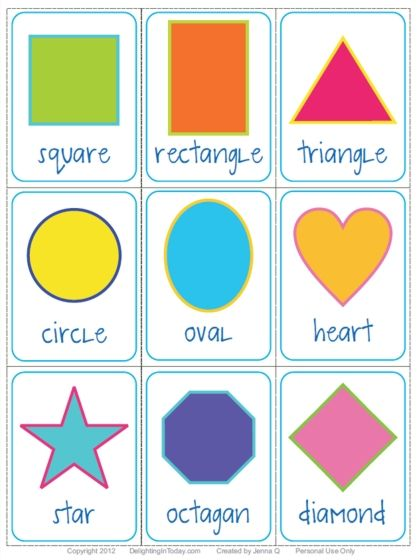
\includegraphics[height=.55\textheight]{images/samples/shapes_supervised}
					\caption*{Exemple de problème d'apprentissage supervisé: les classes (formes géométriques) sont données.}
				\end{figure}
			\end{frame}

			\begin{frame}{Apprentissage supervisé}
				Comment décrire les observations en forme de vecteur?
				\begin{itemize}
					\item<2-> nombre de côtés;
					\item<3-> nombre de sommets;
					\item<4-> convexité;
					\item<5-> symmetrie par rotation;
					\item<6-> \dots;
				\end{itemize}
				\uncover<7->{
					Pour une observation, dont la forme (classe) est un carré, le vecteur d'attributs s'écrit:
					\[\begin{pmatrix}
						4\\
						4\\
						True\\
						False\\
						\vdots
					\end{pmatrix}\]
				}
			\end{frame}

			\begin{frame}{Apprentissage supervisé}
				\begin{figure}[H]
					\begin{center}
						\includestandalone[mode=buildnew, height=.5\textheight]{scatter_gender_dataset}
						\caption*{\tiny Exemple de problème de classification supervisé: 2 attributs et 2 classes.}
					\end{center}
				\end{figure}
			\end{frame}

			\begin{frame}{Apprentissage non-supervisé}
				\begin{itemize}
					\item<1-> Dans le cas de l'apprentissage non-supervisé, on n'observe que les objets à classer, représentés par leurs attributs \(\big(X^i\big)_{i=1,\dots, n}\);
					\item<2-> Le but est de partitionner les instances en groupes (ou clusters) homgènes se ``ressemblent'' en un seul cluster;
					\item<3-> La ressemblance est basée sur les distances dans l'espace des attributs;
					\item<4-> La partition guarantie:
						\begin{itemize}
							\item<5-> des distances faibles intra-cluster;
							\item<6-> des distances grandes intra-cluster.
						\end{itemize}
				\end{itemize}
			\end{frame}

			\begin{frame}{Apprentissage non-supervisé}
				\begin{figure}[H]
					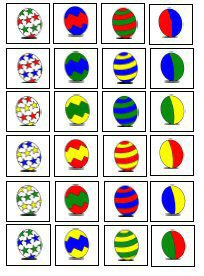
\includegraphics[height=.6\textheight]{images/samples/easter_non_supervised}
					\caption*{Exemple de problématique d'apprentissage non-supervisé.}
				\end{figure}
			\end{frame}

			\begin{frame}{Apprentissage supervisé}
				Comment décrire les observations en forme de vecteur?
				\begin{itemize}
					\item<2-> nombre de côté du motif régulier;
					\item<3-> couleur rouge;
					\item<4-> couleur verte;
					\item<5-> couleur blanche;
					\item<6-> couleur bleue;
					\item<7-> couleur jaune;
					\item<8-> couleur orange;
					\item<9-> convexité du motif;
					\item<10-> symmetrie par rotation du motif;
					\item<11-> symmetrie par translation du motif;
					\item<12-> \dots;
				\end{itemize}
				\uncover<13->{
					Pour l'instance en haut à droite, le vecteur d'attributs s'écrit:
					\[\begin{pmatrix}
						5 & 1 & 1 & 1 & 0 & 0 & 0 & False & False & False \dots
					\end{pmatrix}^T\]
				}
			\end{frame}

			\begin{frame}{Apprentissage non-supervisé}
				\begin{figure}[H]
					\begin{center}
						\includestandalone[mode=buildnew, height=.5\textheight]{scatter_circles}
						\caption*{\tiny Exemple de problème non-supervisé: 2 attributs. Les classes ne sont pas données mais une structure se dégage.}
					\end{center}
				\end{figure}
			\end{frame}

			\begin{frame}{Apprentissage non-supervisé}
				\begin{figure}[H]
					\begin{center}
						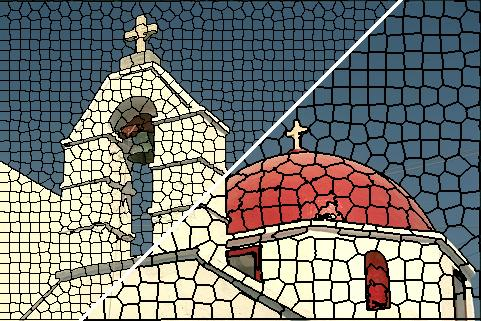
\includegraphics[height=.5\textheight]{images/samples/superpixels}
						\caption*{\tiny Exemple de problème non-supervisé: super-pixelisation d'une image~\cite{achanta2012slic}.}
					\end{center}
				\end{figure}
			\end{frame}
	\section{Algorithmes non-supervisé}
		\subsection{L'inertie}
			\begin{frame}{Disparité intra-cluster}
				\begin{itemize}
					\item<1-> Soit \(\big(S_k\big)_{k = 1, \dots, K}\) une \(K\)-partition de \(\{1, 2, \dots, n\}\).
					\item<2-> Pour chaque sous-ensemble \(S_k\), on définit la quantité \(\sum_{i\in S_k} d(X^i, \mu_k)^2\) où:
						\begin{itemize}
							\item<3-> \(d: \mathbb{R}^d \times \mathbb{R}^d \rightarrow \mathbb{R}_+\) représente une distance: ex. \(d(x, y) = \lVert x - y \rVert\);
							\item<3-> \(\mu_k\) est le barycentre de \(S_k\): \( \mu_k \triangleq \frac{1}{\vert S_k \vert}.\sum_{i\in S_k} X^i\).
						\end{itemize}
					\item<4-> Cette quantité exprime la disparité intra-cluster.
				\end{itemize}
			\end{frame}

			\begin{frame}{Inertie intraclasse}
				\begin{itemize}
					\item<1-> On somme les différentes disparités intra-cluster sur tout les sous-ensembles \(S_k\). On définit l'inertie intraclasse de la partition:
						\begin{equation}
							I_W(\big(S_k\big)_{k = 1, \dots, K}) \triangleq \sum_{k= 1}^{K} \sum_{i\in S_k} d(X^i, \mu_k)^2
						\end{equation}
					\item<2-> Pour le cas particulier de \(K=1\), on vérifie \(\big(S_k\big)_{k = 1, \dots, K} = (\{1,\dots,n\})\). On définit donc l'inertie totale des instances:
						\begin{equation}
							I_T \triangleq \sum_{i=1}^{n} d(X^i, \mu)^2
						\end{equation}
						avec \(\mu = \frac{1}{n} . \sum_{i=1}^{n} X^i\).
				\end{itemize}
			\end{frame}

			\begin{frame}[allowframebreaks]{Inertie totale}
				\begin{align*}
					I_T &= \sum_{i=1}^{n} \lVert X^i - \mu \rVert^2\\
						&= \sum_{k= 1}^{K} \sum_{i\in S_k} \lVert X^i - \mu \rVert^2\\
						&= \sum_{k= 1}^{K} \sum_{i\in S_k} \lVert X^i - \mu_k \rVert^2 + \lVert \mu_k - \mu \rVert^2 + 2. \langle X^i-\mu_k, \mu_k-\mu \rangle\\
						&= I_W(\big(S_k\big)_{k = 1, \dots, K}) + \sum_{k= 1}^{K} \sum_{i\in S_k} \lVert \mu_k - \mu \rVert^2 + 2 . \sum_{k= 1}^{K} \sum_{i\in S_k} \langle X^i-\mu_k, \mu_k-\mu \rangle\\
						&= I_W(\big(S_k\big)_{k = 1, \dots, K}) + \sum_{k= 1}^{K} \vert S_k \vert \lVert \mu_k - \mu \rVert^2 + 2 . \sum_{k= 1}^{K} \langle \sum_{i\in S_k} (X^i-\mu_k), \mu_k-\mu \rangle
				\end{align*}
				\begin{align*}
					I_T &= I_W(\big(S_k\big)_{k = 1, \dots, K}) + \sum_{k= 1}^{K} \vert S_k \vert \lVert \mu_k - \mu \rVert^2 + 2 . \sum_{k= 1}^{K} \langle \sum_{i\in S_k} X^i - \vert S_k \vert . \mu_k, \mu_k-\mu \rangle\\
						&= I_W(\big(S_k\big)_{k = 1, \dots, K}) + \sum_{k= 1}^{K} \vert S_k \vert \lVert \mu_k - \mu \rVert^2 + 2 . \sum_{k= 1}^{K} \langle \sum_{i\in S_k} X^i - \vert S_k \vert . \frac{1}{\vert S_k \vert} . \sum_{i\in S_k} X^i, \mu_k-\mu \rangle\\
						&= I_W(\big(S_k\big)_{k = 1, \dots, K}) + \sum_{k= 1}^{K} \vert S_k \vert \lVert \mu_k - \mu \rVert^2
				\end{align*}
			\end{frame}

			\begin{frame}{Inertie interclasse}
				\begin{itemize}
					\item<1-> On définit ainsi l'inertie interclasse:
						\begin{equation}
							I_B(\big(S_k\big)_{k = 1, \dots, K}) = \sum_{k= 1}^{K} \vert S_k \vert \lVert \mu_k - \mu \rVert^2
						\end{equation}
						on a donc:
						\begin{equation}
							I_T = I_B(\big(S_k\big)_{k = 1, \dots, K}) + I_W(\big(S_k\big)_{k = 1, \dots, K})
						\end{equation}
					\item<2-> Cette quantité exprime la disparité entre les barycentre de cluster et le barycentre de tous les échantillons. Plus elle est grande, plus l'hétérogénité de la partition est grande.
					\item<3-> Puisque \(I_T\) est constante, minimiser la disparité intra-cluster \(I_W\) revient à maximiser \(I_B\).
					\item<4-> Trouver la meilleure partition revient à résoudre le problème:
						\begin{equation}
							\arg \min_{\substack{K = 1,\dots,n \\ \big(S_k\big)_{k = 1, \dots, K}}} I_W(\big(S_k\big)_{k = 1, \dots, K})
						\end{equation}
				\end{itemize}
			\end{frame}

			\begin{frame}{Combinatoire}
				\begin{itemize}
					\item<1-> A premier abord, on peut essayer toutes les partitions possibles.
					\item<2-> Pour \(n\) instances et \(K\) classes, le nombre totale de partition~\cite{StirlingWiki}:
						\begin{equation}
							S_{n,K} \triangleq \left\{ {n \atop k}\right\} = \frac{1}{k!}\sum_{j=0}^{k} (-1)^{k-j} \binom{k}{j} j^n
						\end{equation}
					\item<3-> Pour \(k \neq 1, n\):
						\begin{equation}
							S_{n,K} \underset{n\infty}{\sim} \frac{K^n}{K!}
						\end{equation}
					\item<4-> Pour toute les partitions possibles, on dénombre:
						\begin{equation}
							B_n \triangleq \sum_{k=0}^n \left\{ {n \atop k}\right\} = \frac{1}{e}\sum_{k\in\mathbb{N}} \frac{k^n}{k!}
						\end{equation}
						avec: \(\frac{B_n}{n^n} \underset{n\infty}{\sim} 1\)~\cite{BellWiki}.
				\end{itemize}
			\end{frame}
		\subsection{Clustering hiérarchique}
			\begin{frame}{Clustering hiérarchique}
				\begin{itemize}
					\item<1-> On repose sur la métrique \(d\) qui repose sur la géométrie dans l'espace des attributs.
					\item<2-> On définit une distance entre clusters:
						\begin{itemize}
							\item<3-> \(D_m: (A, B) \mapsto \min_{a\in A, b\in B} d(a,b)\)
							\item<4-> \(D_M: (A, B) \mapsto \max_{a\in A, b\in B} d(a,b)\)
							\item<5-> \(D_b: (A, B) \mapsto \frac{1}{\vert A \vert.\vert B \vert}\sum_{a\in A, b\in B} d(a,b)\)
							\item<6-> \dots
						\end{itemize}
					\item<7-> On regroupe (\textit{resp.} divise) les clusters qui vérifient le minimum (\textit{resp.} maximum) de distance~\cite{hastie2009unsupervised,ward1963hierarchical}.
				\end{itemize}
			\end{frame}
			\begin{frame}{Algorithme}
				\begin{algorithm}[H]
					\KwData{Les observations: \(\big(X^i\big)_{i=1,\dots,n}\)}
					\KwData{La métrique de l'espace: \(d: \mathbb{R}^d \times \mathbb{R}^d \rightarrow \mathbb{R}_+\)}
					\KwData{La métrique de cluster: \(D: 2^{\{X^i: i=1,\dots,n\}} \times 2^{\{X^i: i=1,\dots,n\}} \rightarrow \mathbb{R}_+\)}
					\KwData{Le nombre d'itération maximale: \(I\)}
					\KwData{Le nombre de cluster: \(K\)}
					
					\KwResult{La partition: \(\big(S_k\big)_{k=1,\dots,K}\)}
					\(i = 0\), \(S^i_k:=\{X^k\}, \quad \forall k = 1,\dots,n\), \(cl=n\)\;
					\While{\(cl > K\) and \(i < I\)}{
						\(i := i + 1\)\;
						\(\big\{c_1, \dots, c_{p_i}\big\} := \arg\min_{\substack{s=1,\dots,cl\\t=1,\dots,cl}} D(S^{i-1}_s, S^{i-1}_t)\)\;
						\(\{e_1,\dots,e_{q_i}\} := \big\{\bigcup_{\substack{k=1,\dots,p_i\\c_j\cup c_k \neq \emptyset}} c_k: j=1,\dots,p_i\big\}\)\;
						\(\forall k=1,\dots,q_i \quad S^i_k := \bigcup_{j\in e_k} S^{i-1}_j\)\;
						\(\big\{S^i_k: k=q_i+1,\dots,cl\} := \{S^{i-1}_h: h\in\{1,\dots,cl\} \setminus \bigcup_{j=1}^{q_i} e_j \big\}\)\;
						\(cl:= cl + q_i - \sum_{j=1}^{q_i} \vert e_i\vert\)\;
					}
				\end{algorithm}
			\end{frame}

			\begin{frame}{Exemple}
				\begin{figure}[H]
					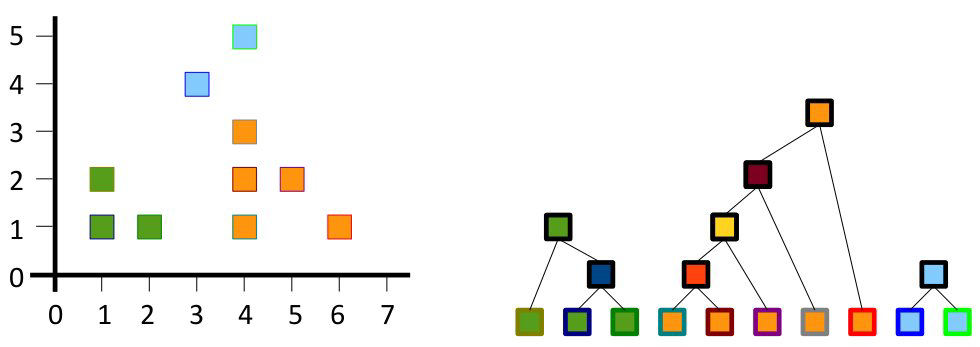
\includegraphics[width=.8\textwidth]{images/samples/hierchical_clustering.png}
					\caption*{Exemple de clustering hiérarchique}
				\end{figure}
			\end{frame}
		\subsection{Clustering avec partitionnement}

	\section{Algorithmes supervisé}
		\subsection{Types de méthodes}
		\subsection{Méthodes génératives}
		\subsection{Méthodes discriminative}
	\section{Références}
	\begin{frame}[allowframebreaks]{Références}
		\nocite{sklearn_api}
		\bibliographystyle{apalike}
		\bibliography{references.bib}
	\end{frame}

\end{document}
